\section{\uppercase{Related Work}} \label{sec:relatedWork} 
\noindent This section is broken into two subsections.  The first briefly
covers the advances made in the field of online failure prediction and how they
relate to our tool, and the second details existing tools for network traffic
generation.

\subsection{Online Failure Prediction}
\noindent In 2010, Salfner et al. published a survey of online failure
prediction techniques that categorized the many approaches that have been
explored into a taxonomy~\cite{salfnerSurvey}.  Many of these failure
prediction techniques are based in machine learning and require steady system
states but sadly, as the software development life-cycle has grown shorter over
time, a steady system state is no longer a guarantee.

Since the publication of Salfner et al.'s survey, it has been pointed out that
while many effective techniques for predicting failure exist, these techniques
are too difficult to maintain and consequently are not being used.  In 2015,
Irrera et al. published a framework called the Adaptive Failure Prediction
(AFP) framework for dealing with this problem that automated the process of
retraining a failure prediction algorithm after an underlying system
change~\cite{irrera2015}.  After a system change, a virtual clone of the
production system is made and then load against this clone is generated.  After
the cloned system is sufficiently loaded, faults are injected which quickly
lead to failure.  This failure is captured, labeled, and used to train a new
predictor.  The new predictor is compared against the old one and replaces it
if the new outperforms the old.

The target system for this research is a Microsoft Windows active directory
domain services server and, as a result, full-stack authenticated session
traffic is required in order to sufficiently load the service.  In this work,
we seek to enable the generalization of the AFP framework and were unable to
find a sufficient load generation tool to carry out the automated retraining of
a predictor defined in AFP.

\subsection{Network Load \& Traffic Generation}

\noindent Many tools exist for the purpose of generating network traffic.
Generally, these tools are classified into three categories: application-level,
flow-level, and packet-level generators~\cite{botta2012,zach2013}.
Application-level generators emulate traffic produced by applications on a
network, flow-level generators replicate actual traffic using statistical
modeling, and packet-level generators create and inject packets into the
network.  Network traffic generators are further classified as open- or
closed-loop.  Open-loop generators use a packet arrival model for packet
timing, whereas closed-loop generators wait for a response to a sent request
prior to sending the next request~\cite{weigle2006}.  Unfortunately, as far as
we can tell, none of the tools available generate the necessary interaction
with a deployed Microsoft Windows active directory environment necessary to
facilitate the implementation of the AFP framework.  Active directory
implements the Kerberos authentication protocol in Windows domains and due to
its cryptographic nature cannot be tested against replayed or random traffic;
rather, a sequence of valid and invalid requests and responses are necessary to
stress test this framework.  Indeed, multi-step ``handshakes'' are necessary
for rich service delivery and this capability is not realized by the current
tools with any degree of modularity or extensibility.

A brief review of the traffic generators considered when researching this
problem follows.  The Distributed Internet Traffic Generator
(D-ITG)~\cite{botta2012} is, as its name implies, a distributed traffic
generator capable of performing application, flow, and packet-level generation
using both open- and closed-loop operations -- sessions are initiated at
specific time intervals and, within each session, new requests are not sent
prior to receiving a response to the previous request.  Sadly, D-ITG currently
only supports TCP, UDP, ICMP, DNS, Telnet and VoIP which does not suit our
needs.

NTG~\cite{zach2013} is an application-level, distributed network traffic
generator which is both open- and closed-loop.  A key feature of NTG, as it
relates to our problem, is that it interacts with existing network services.
Unfortunately, it is only limited to web, mail, and multimedia
servers/services, which is insufficient for our purposes.

Swing~\cite{vishwanath2009} is a flow-level, closed-loop traffic generator that
observes live network traffic, extracts distributions from the traffic, and
generates new traffic in a manner consistent with the observed traffic
distributions.  While this tool provides the ability to generate
statistically-realistic traffic from generators to listeners across a link, the
lack of both two-way traffic and interaction with existing services
(specifically authentication services) does not satisfy the requirements for
our problem.

A final tool worth mentioning, while not a network traffic generator, is
Microsoft's Active Directory Performance Testing Tool
(ADTest)\footnote{\url{https://www.microsoft.com/en-us/download/details.aspx?id=15275}}.
Official Microsoft documentation is limited, however
in~\cite{bijaoui2011,morowczynski2014,suyanto2010,suyanto2010_2} we find that
ADTest assesses the ability of Microsoft 2003/2008/2012 Active Directory
Lightweight Directory Services (AD LDS) servers to add organization units and
users, and make various changes to Active Directory to aid in developing
requirements for an AD LDS deployment.  It is important to note that Microsoft
no longer supports this tool~\cite{morowczynski2014}.  Also of importance,
ADTest is not capable of testing other services that rely on active directory
domain services for authentication (e.g. RDP, SMB, etc), nor can it be extended
to do so, and is therefore insufficient for our goals.

While all of these tools are, in general, sufficient for generating traffic in
a network, they do not generate full-stack, two-way authentication that is
needed in order to sufficiently load the active directory domain services
service.  Further, these tools work by replaying traffic transactions that have
already taken place and as a result, this type of traffic cannot be used to
force any network services to do any meaningful or realistic work.  The AFP
requires the target system be placed under realistic load before injecting
faults to capture the most realistic failure data
possible~\cite{irrera2014,irrera2015}.  Due to the nature of the authentication
protocols used in enterprise domains, it is not possible to realistically
generate this traffic without valid user credentials and a dynamic
authentication session that cannot be replayed due to its cryptographic nature.
A tool to generate this type of traffic did not previously exist.

\section{\uppercase{Distributed PowerShell Load Generator (D-PLG)}}
\label{sec:contrib} 
\noindent We present D-PLG, a new tool for the generation of realistic network
traffic in a Microsoft Windows domain for the purposes of software testing or
load generation.  D-PLG can be classified as an application-level closed loop
traffic generator and is a basic Windows PowerShell script that uses native
PowerShell cmdlets for all of its functionality ensuring that the most
realistic traffic possible is generated without overburdening the client
machines used for generating load.  D-PLG offers what has not seen in other
traffic generation products or tools by making actual service requests and
producing actual challenges and responses for Windows authentication protocols.

D-PLG is written in the Windows PowerShell environment because it provides a
tremendous amount of power and flexibility to generate traffic that would
actually be generated by a users interaction with network services since the
same software applications and libraries are used.  As a result, D-PLG does
require the use of client machines. However, this work does show that
generating this type of realistic traffic is possible by utilizing only a small
number of machines, or without producing a noticeable burden on in-use client
machines.

\begin{figure}[!ht] \centering 
    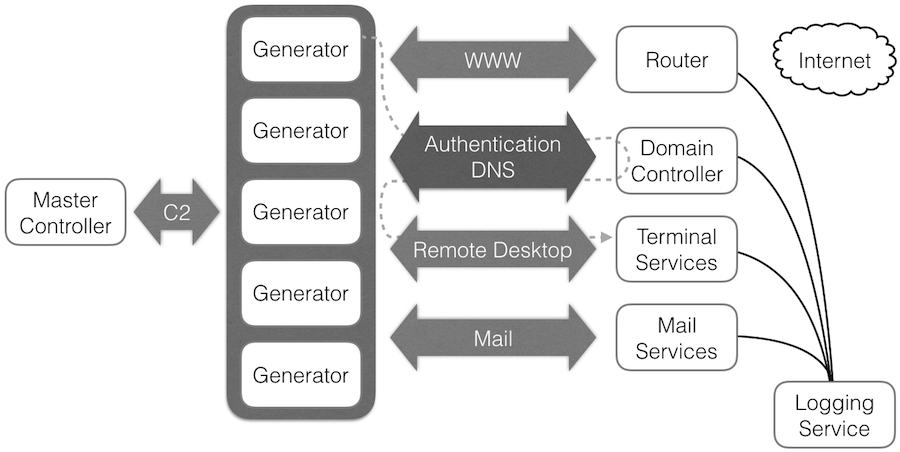
\includegraphics[width=2.8in]{ConceptDiagram}
    \caption[Concept Diagram]{How each type of traffic that is generated is
    routed.  Log events are offloaded to logging service for further analysis.}
    \label{fig:conceptDiagram} 
\end{figure}

In general, the intended architecture can be seen in
Figure~\ref{fig:conceptDiagram}.  D-PLG is most effective if used by a few
client machines during idle downtimes but is developed in such a way that a
user can still use a machine that is generating load, but may notice degraded
performance depending upon how much traffic that particular client is being
asked to generate.  D-PLG is currently designed to run from one central
location, asking a configurable list of clients to produce traffic for a fixed
period of time.  

It should be noted that D-PLG implements a feature that has not been previously
seen and thus, a comparison with the existing tools is difficult.  Relevant
existing tools simply replay previously observed traffic which may be more
representative of realistic load, but are incapable of creating any real work
for cryptographic system.  Modern cryptography relies on random and dynamic
challenge-response protocols, as a result any inbound requests that are not
capable of generating dynamic challenge responses are typically dropped
immediately.

In its present form, D-PLG is comprised of three modules capable of generating
full-stack web requests, Microsoft remote desktop protocol, Microsoft server
message block (SMB) file sharing, and all associated authentication traffic.
An intended byproduct of all of this traffic is domain name system (DNS)
requests.  An important part of any active directory domain is DNS and as a
result, no load generator would be complete without performing DNS lookups.

The rest of this section outlines each of the three modules currently
implemented as well as our plans for future modules.

\subsection{Web Browsing} 
\noindent D-PLG is capable of generating full-stack web requests and presently
simulates an actual user browsing.  This module is implemented using the
`Invoke-WebRequest' PowerShell cmdlet which upon completion returns an object
representing the full document object model (DOM).  The return of this object
allows us to programmatically simulate random browsing within a returned page.
As a result, our tool is capable of generating realistic web traffic against a
web server.  This functionality is different from the functionality implemented
in many of the existing tools that only generate one-way transmission of the
web request.  As a result, this module allows users of our tool to generate
realistic load against web servers and potentially automate realistic web
application testing.

The web browser was created with minimal effort as our approach to D-PLG
emphasizes rapid generation of modern internet-based interactions.  In future
versions, we plan to implement more dynamic web browsing to facilitate the use
of D-PLG as an automated web application testing tool.  Since the entire DOM is
returned, it is possible and relatively simple to programmatically complete web
forms, and submit REST API calls in only a few lines of PowerShell code.
 
\subsection{Remote Desktop Protocol} 
\noindent Remote Desktop Protocol (RDP) is a simple protocol that allows the
sharing and remote control of a Windows desktop environment.  This module was
included to generate more authentication traffic with our active directory
domain services server as well as place load on our remote desktop services
server.  Applications for this module could include network infrastructure
capacity and server sizing planning.  The module takes advantage of a modified
third party cmdlet~\cite{brasser15} which invokes a call to the native windows
remote desktop application (mstsc.exe).  Our modification only tells the cmdlet
not to present a window as to avoid interrupting an individual who may be using
the computer at the time of load generation.

Currently, the RDP module makes a full-stack remote desktop connection with an
RDP server without producing a window which can allow us to take advantage of
clients in active states.  The script then sleeps for a few seconds and then
closes the connection.  In future versions, we would like to implement some
sort of actual interaction with the RDP server like file upload or application
use.  This functionality was based on a tool previously developed by
Microsoft\footnote{\url{https://www.microsoft.com/en-us/download/details.aspx?id=2218}}
which is no longer maintained as evidenced here~\cite{szeto12}.

\subsection{Server Message Block (SMB) File Sharing}
\noindent D-PLG implements an SMB file sharing module that connects to a local
or remote share, creates a file in the share, fills that file with random ASCII
data, saves the file, deletes the file, and finally deletes the share.  This
sequence of operations ensures that full-stack SMB file sharing requests are
utilized and thus, causing the domain services server to authenticate the
transaction and the file sharing services server to process the data being
uploaded.  This simple module could additionally be used to ensure a file
server is live before beginning more complex operations.

Like the previous module, the SMB module was rapidly built due to the
flexibility of our framework and implemented in only fourteen lines of code.
In future versions, we plan to implement a variable amount of upload data or
allow the user to select his or her own file.  By allowing the user to upload a
custom file, this module could be used to test application aware firewall rules
to ensure certain types of files are or are not allowed to traverse a network.

\subsection{Future Modules} 
\noindent We have already implemented many core active directory domain
services as a proof of concept, but would like to point out how easy additional
services would be to implement in our script.  For example, simple message
transfer protocol (SMTP) traffic could be implemented in a single line of
PowerShell code using the `Send-MailMessage' cmdlet.  Additionally, the
`Out-Printer' cmdlet would allow for the sending of realistic full-stack
network printer traffic.  To facilitate future development, we have published
D-PLG in its current form under the MIT license on
GitHub\footnote{\url{https://github.com/paullj1/afp-dc/tree/master/D-PLG}}.

These modules demonstrate our platforms extensibility and are representative of
sophisticated network interactions that are necessary to create a performant
load generator for the tableau of modern networking services.  

\section{\uppercase{Methodology}} \label{sec:methodology} 
\noindent This section is split into two subsections.  In the first, we
describe in detail our virtual environment.  In the following section, we
detail the design of our experiments which utilized our virtual environment.

\subsection{Virtual Environment}
\noindent The virtual environment was hosted on two VMWare ESXi 5.5 hypervisors
each with two 2.6 GHz AMD Opteron 4180 (6 cores each) CPUs and 64 GB memory.
The individual virtual machines are detailed in Tables~\ref{fig:hyp1},
and~\ref{fig:hyp2}.  D-PLG uses cmdlets that did not exist until PowerShell
version 3.0 so each of the Microsoft (MS) Windows computers had the MS Windows
Management Framework version 4.5 installed.  The installation of this framework
also necessitated the installation of the MS .NET Framework version 4.5.  In an
enterprise environment these software frameworks would more than likely already
be installed as they are part of the service pack updates that have since been
released by Microsoft.

\begin{table}[!ht] \centering
  \caption{Hypervisor 1.}
  \begin{tabular}{ | c | l | l | c | l |}
    \hline
    Qty. & Role   & Operating System & CPU / Mem. \\ \hline\hline
    1    & DC     & Win. Server 2008 & 2 / 2 GB   \\ \hline
    5    & Client & Win. 7           & 1 / 512 MB \\ 
    \hline
  \end{tabular}
  \label{fig:hyp1}
\end{table}

\begin{table}[!ht] \centering
  \caption{Hypervisor 2.}
  \begin{tabular}{ | c | l | l | c | l |}
    \hline
    Qty. & Role & Operating System & CPU / Mem. \\ \hline\hline
    1    & RDP  & Win. Server 2008 & 1 / 4 GB   \\ \hline
    1    & Log  & Ubuntu 14.04 LTS & 1 / 1 GB   \\ 
    \hline
  \end{tabular}
  \label{fig:hyp2}
\end{table}

After installing the requisite software, each client was added to the domain
and required a few minor modifications.  First, D-PLG creates remote
`PSSessions' on each client machine and then invokes the cmdlets that have been
assembled to generate the desired load.  In order for this to happen, the
credentials of the controller must be delegated so that they may be used to
make the connections through the PSSession.  This delegation is done very
simply through the PowerShell cmdlet `Enable-WSManCredSSP'.  The final
modification was for convenience; a copy of the scripts to be executed remotely
was placed on the desktop of the Administrator user.

The domain controller had two MS Windows Server roles enabled: active directory
domain services, and domain name service (DNS).  One domain administrator
account was used for command and control traffic, and individual user accounts
were created and used for RDP and simple authentication traffic.  The RDP
server only had one MS Windows Server role enabled: remote desktop services.

The Ubuntu server was deployed and used as a central log repository for
analyzing load on the domain controller and RDP server.  The default rsyslog
application was simply configured to accept incoming connections and then the
rsyslog Windows agent was installed on the domain controller and RDP server.

D-PLG is divided into two scripts.  The first is the `LocalLoadGen' script
and is placed on each client computer.  We note here that placing the script on
the each client computer may not be ideal in a production environment and this
step could easily be automated when the controller runs.  Further, upon
completion, the script could be removed in a single PowerShell command.  The
second script `RunLoadSim' is designed to act as a command and control element
that connects to each client and executes the `LocalLoadGen' script as an
asynchronous job.  In our experiments, the command and control script was
executed from our RDP server. 

\subsection{Experiment Design} \label{sec:experimentDesign}
\noindent Two experiments were designed to test and demonstrate the efficacy
of our tool and are detailed here.  In both of the following tests, D-PLG was
run five times, where each execution consisted of five minutes of traffic
generation within our virtual environment.  The domain controller was sized
based on Microsoft's community recommendation for up to fifteen thousand users
in~\cite{mak12}.  Our goal was to produce a sufficient enough amount of traffic
to achieve the level of load that was suggested our server be able to sustain
based on how it was sized.  To determine if that goal was achieved, ESXi's
reporting tools were used to collect the relevant data in the form of packet
captures at the virtual switchports of one client machine, the terminal server,
and the domain controller.  Further data collected came from the ESXi
performance data.  After each round of our tests, the performance data were
exported from each of the hypervisors on the terminal server, one client, and
the domain controller.  In these data, CPU utilization, memory utilization,
disk operations, and network traffic are reported on twenty second intervals.
Finally, as previously stated, the rsyslog Windows Agent was used to forward
the logs from the domain controller and RDP server to an Ubuntu server.  These
log entries were then split into pieces that corresponded with each round of
the tests.

The first question we wanted to answer was, how much traffic can a PowerShell
script really generate, and is it enough to sufficiently load an enterprise
domain controller?  The first experiment was designed to answer that question.
To maximize the amount of traffic and subsequent load generated, the client
machines were only configured to make a single request.  To do this, the
`RunLoadSim' was only tasked to perform a basic authentication request to the
domain controller.  The goal was to maximize the number of authentication
requests the server could handle based on the way it was sized.  In our case,
that number was fifteen thousand users and a goal CPU utilization of 40\%.  To
prevent overburdening the client machines, we found that the highest frequency
at which these events could be created and handled was 10 per second.
Fortunately, five clients running for five minutes making ten requests per
second equated to exactly fifteen thousand requests.  

It should be noted here that the client machines used were significantly less
powerful than average desktop computers typically found in an enterprise
environment.  Each authentication event took 20 milliseconds so the maximum
number of requests per second that was observed was fifty.  As a result, this
same experimental setup can sufficiently load a domain controller sized for
seventy-five thousand users.

In the second experiment we wanted to determine how much load could be produced
without having a significant effect on the resources available to each client
machine.  We configured the clients to utilize each of the modules that are
currently implemented in D-PLG.  In each round of the test the client machines
looped continuously making an authentication request to the domain controller,
a full RDP connection, an SMB share connection, a web request to a randomly
selected URL, and finally a web request to a URL randomly selected from the
page returned by the first request.  The loop was configured to run twice per
second, however due to the high latency of the web requests, the client was not
expected to make that many requests every second of the test.  This
configuration choice was made to ensure maximum utilization when possible.

\section{\uppercase{Experimental Results}} \label{sec:results}
\noindent In this section the results and data collected after conducting the
tests described in Section~\ref{sec:experimentDesign} are detailed.  To answer
the quantity question, the number of packets produced per second was explored
as well as CPU utilization, memory utilization, log events, and network
operations on the domain controller.  In this first round of tests, the domain
controller reported an average of 56,291 log events over each five minute test
or approximately 187 log events per second.  In addition, an average of 6,267
packets per second were captured over each of the five tests.
Figure~\ref{fig:authDCPPS} shows the distribution on the number of packets sent
and received by the domain controller for each test and tells us that the load
was consistently high throughout each test.  On the client side, as we
predicted, the load was also relatively high as seen in
Figure~\ref{fig:authClientMetrics}.

\begin{figure}[!ht] \centering
  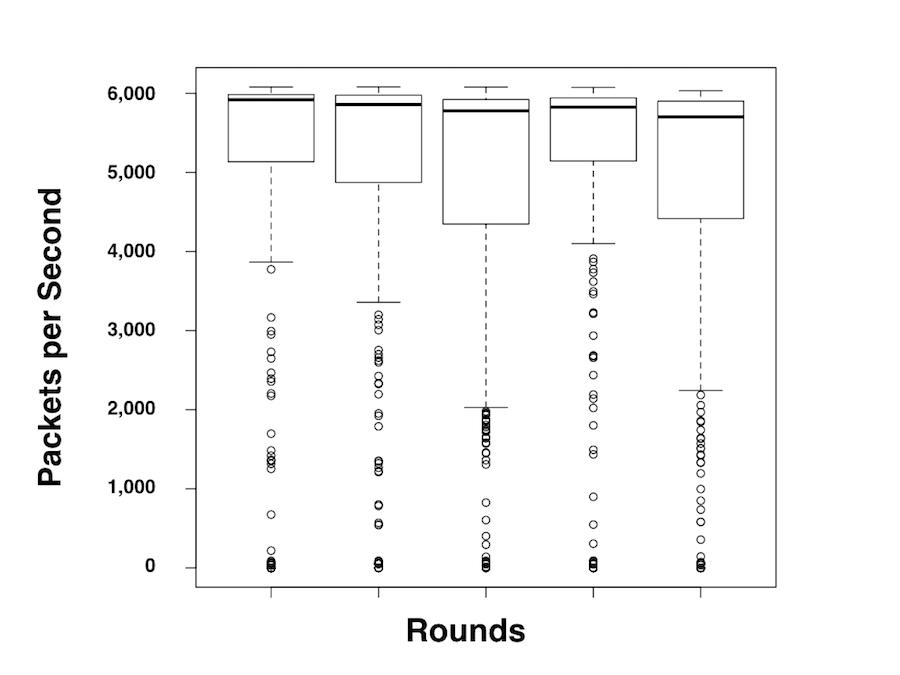
\includegraphics[width=3in]{authDCPPS}
  \caption[Domain Controller Packets per Second]{How many packets per second
  were sent or received by the domain controller across all five rounds of the
  first test.  In each test, approximately 1.8 million packets were captured.}
  \label{fig:authDCPPS}
\end{figure}

\begin{figure}[!ht] \centering
  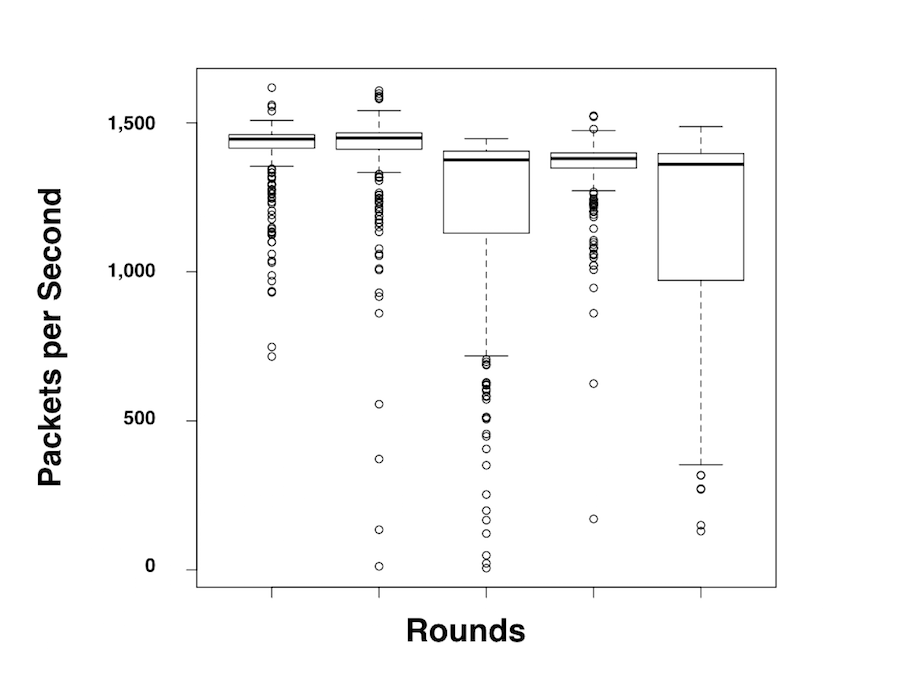
\includegraphics[width=3in]{authClientPPS}
  \caption[Client Packets per Second]{How many packets per second were sent or
  received by one of the clients across all five rounds of the first test.}
  \label{fig:authClientPPS}
\end{figure}

\begin{figure}[!ht] \centering
  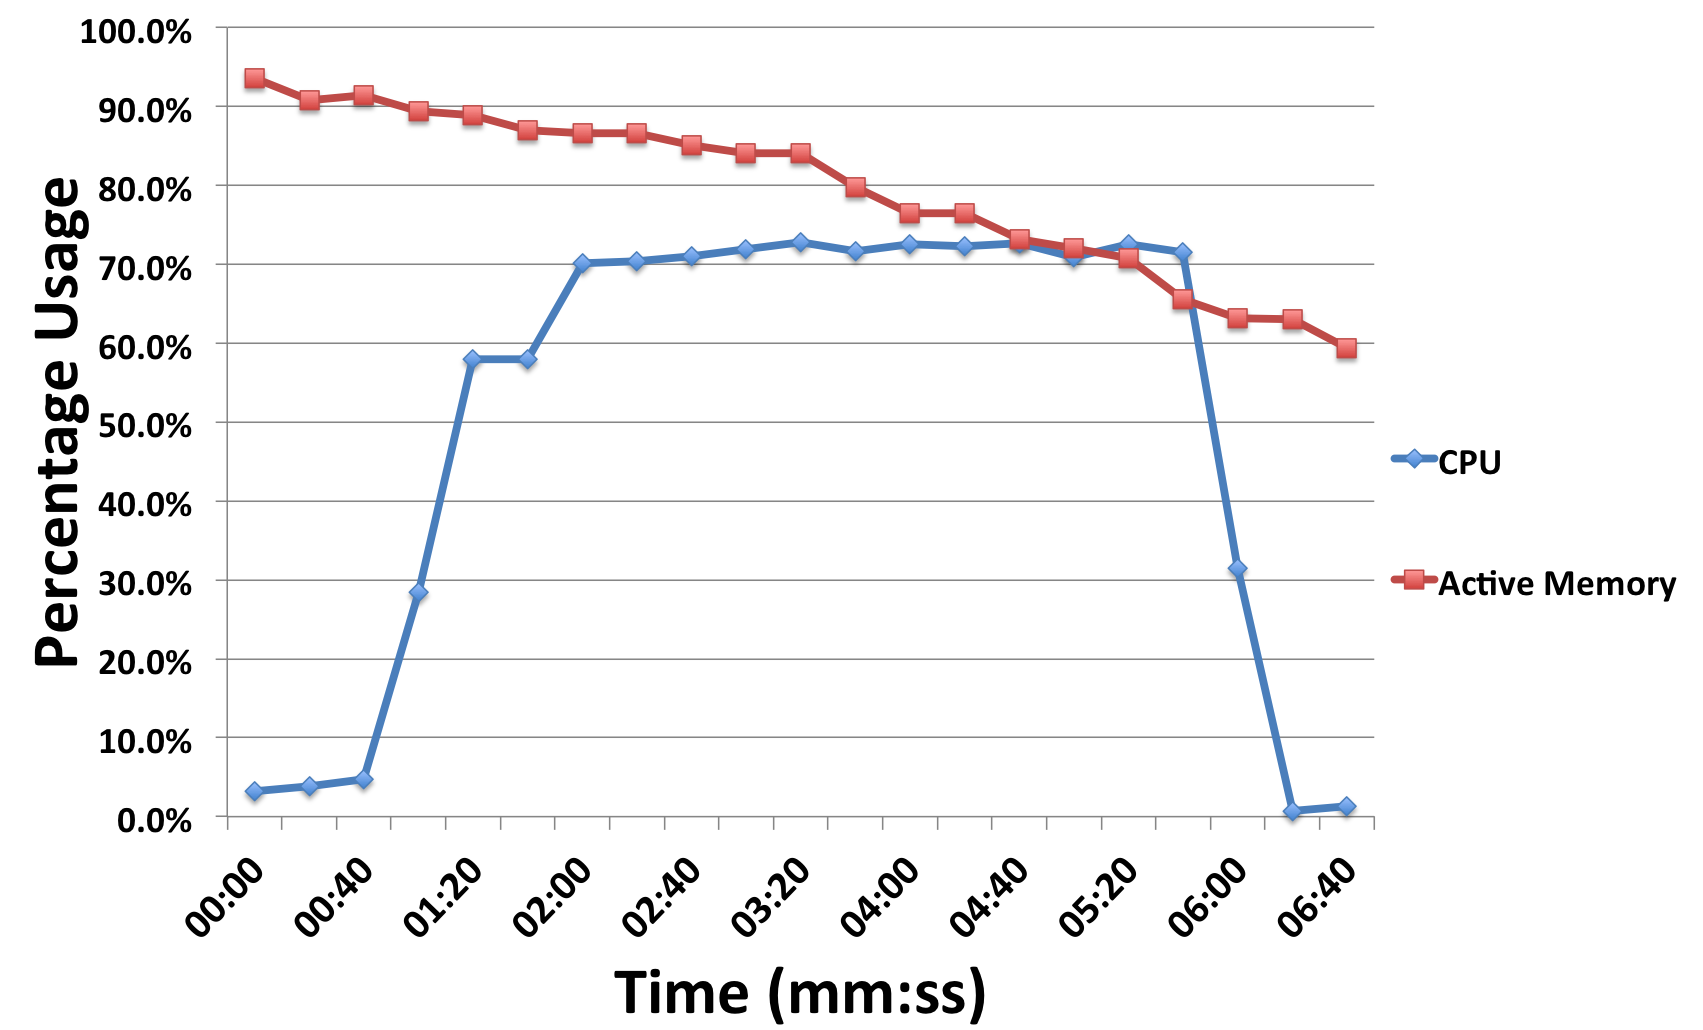
\includegraphics[width=2.8in]{authClientMetrics}
  \caption[Test 1:  Client Metrics]{Client CPU and memory utilization during
  the first test.}
  \label{fig:authClientMetrics}
\end{figure}

\begin{figure}[!ht] \centering
  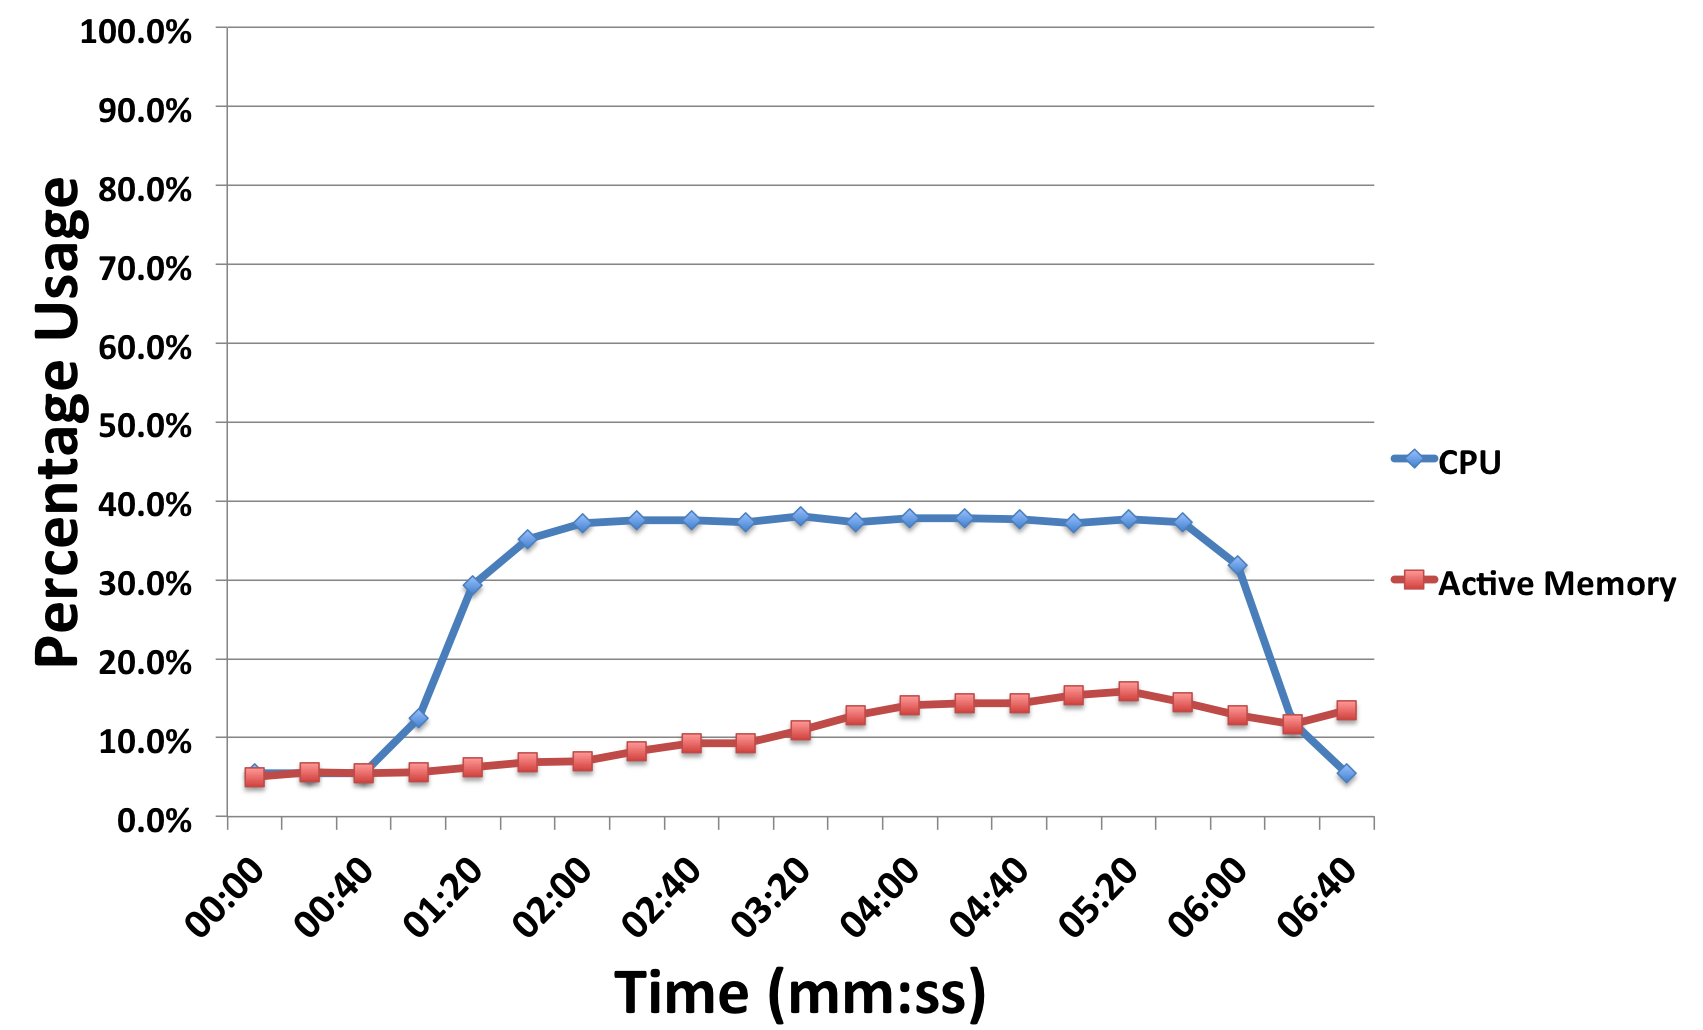
\includegraphics[width=2.8in]{authDCMetrics}
  \caption[Test 1:  Domain Controller Metrics]{Domain controller CPU and memory
  utilization during the first test.}
  \label{fig:authDCMetrics}
\end{figure}

These results validate our hypothesis.  The load generated against the domain
controller was consistently at 40\% which is exactly in-line with the amount of
load it should be expected to endure during peak business hours per the
Microsoft community recommendations for sizing~\cite{mak12}.  Unfortunately in
this case, the client machines would likely not have been usable during the
test.  Fortunately, because only five low-end are needed machines to produce
this load over a relatively short period of time, a simple solution to this
problem would be to purchase five inexpensive desktop computers for this
purpose, or conduct testing during an idle downtime.

In the second test, we were trying to find out if the client machines could
produce a sufficient amount of realistic traffic without being over burdened so
that they could be used to generate load even as individuals use them.  To
answer this question we examined CPU and memory utilization, and packets
transmitted per second with respect to the client.  The average number of
packets generated over the five minute tests was 5,499 and the remainder of
the data can be seen in Figure~\ref{fig:allModsClientMetrics}.  We also
examined these same data with respect to the domain controller and RDP server
seen in Figures~\ref{fig:allModsDCMetrics}, and~\ref{fig:allModsRDPMetrics}
respectively.

\begin{figure}[!ht] \centering
  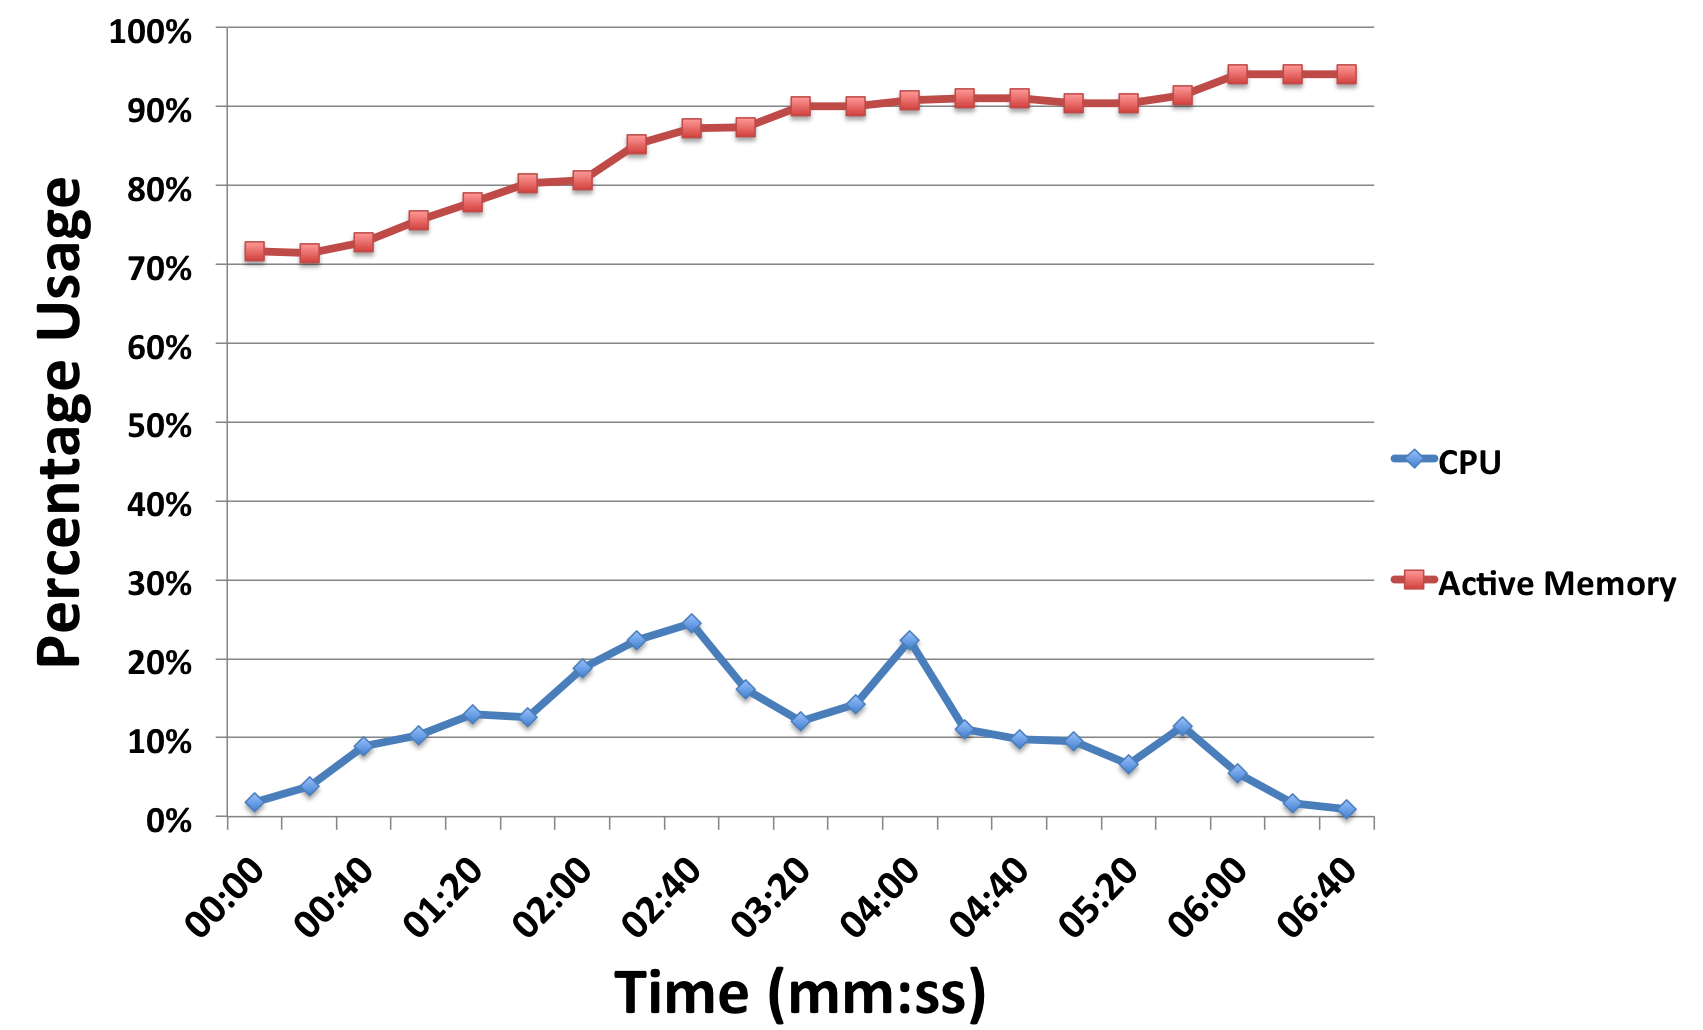
\includegraphics[width=2.8in]{allModsClientMetrics}
  \caption[Test 2:  Client Metrics]{Client CPU and memory utilization during
  the second test.}
  \label{fig:allModsClientMetrics}
\end{figure}

\begin{figure}[!ht] \centering
  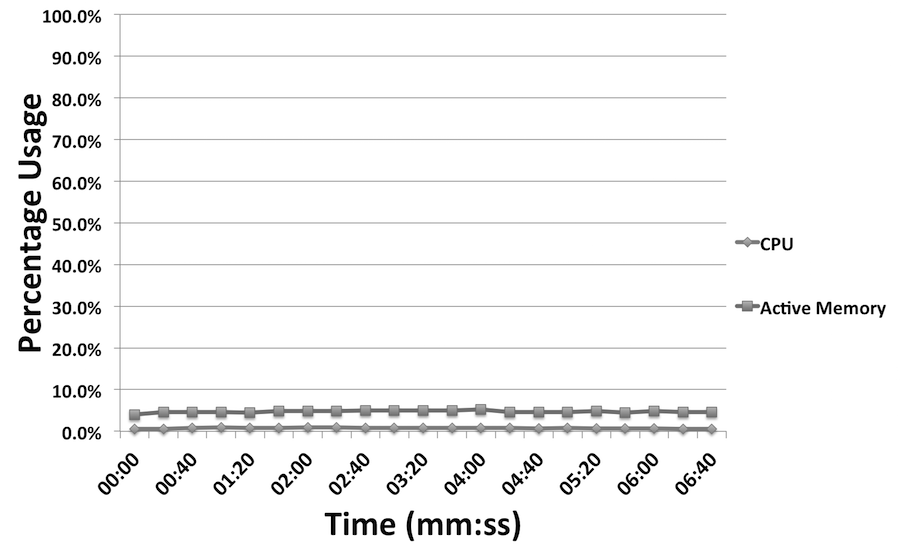
\includegraphics[width=2.8in]{allModsDCMetrics}
  \caption[Test 2:  Domain Controller Metrics]{Domain controller CPU and memory
  utilization during the second test.}
  \label{fig:allModsDCMetrics}
\end{figure}

\begin{figure}[!ht] \centering
  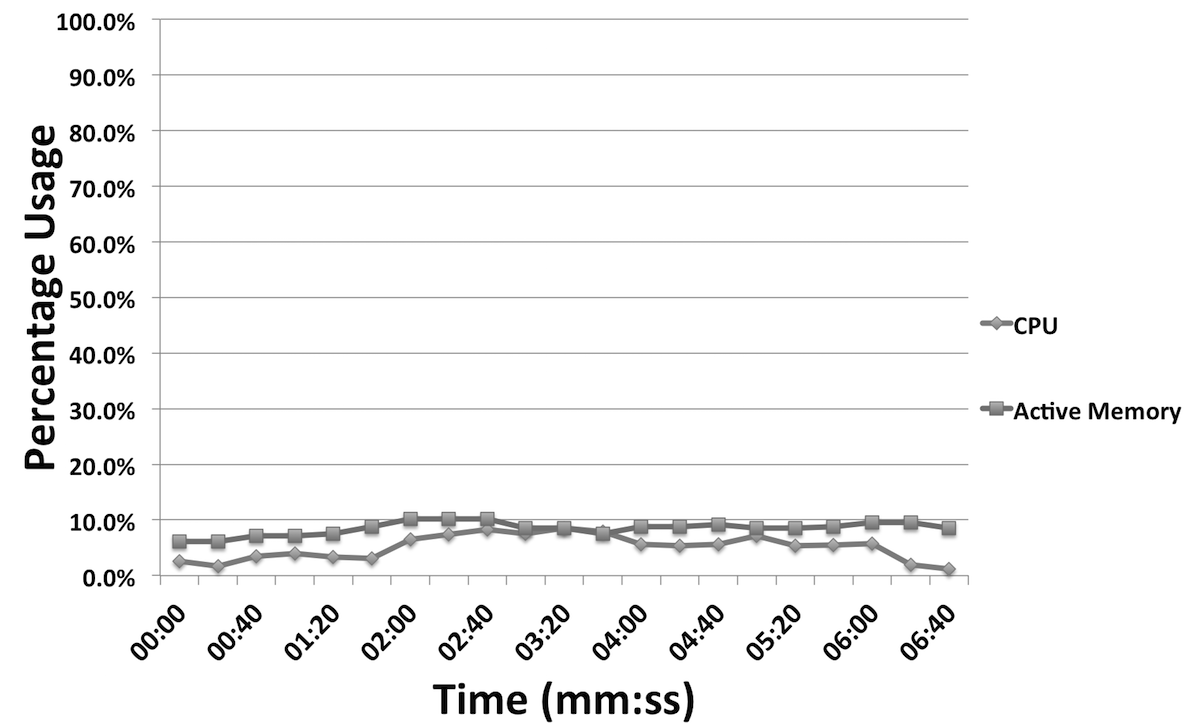
\includegraphics[width=2.8in]{allModsRDPMetrics}
  \caption[Test 2: RDP Metrics]{RDP server CPU and memory utilization during
  the second test.}
  \label{fig:allModsRDPMetrics}
\end{figure}

While the number of packets was relatively high, these results do not
demonstrate a sufficient amount of load on either the domain controller or RDP
server.  We suspect that this is due to the majority of the time spent during
the test retrieving web-pages.  As a result, if a proxy server or application
aware firewall is the target of this load generation, this level of traffic is
sufficient for that purpose.  These results also show that a client computer
asked to generate traffic could still be used during a test.  In future work,
we plan to test this infrastructure with non-blocking web-requests so that more
load can be placed against the local services while web requests are being
processed externally.  Alternatively, more client machines could be used during
the test.

In general, the results observed lead us to believe that our tool can be
extended and used under any circumstance where dynamic network transactions are
required between unbounded network components.  Further, these results show
that our tool will allow us to leverage the AFP framework in our future work.

\section{\uppercase{Future Work}} \label{sec:futureWork}
\noindent There are many opportunities for improvement in D-PLG.  If D-PLG is
to be used to simulate realistic network traffic patterns that would normally
be generated by humans, much work would have to be done to balance the kinds of
requests that get made.  For example, a typical user might log in, browse the
web for a few minutes, check his or her e-mail, then maybe send an e-mail.
Currently, D-PLG is extremely predictable with respect to what kind of request
it will make next.  The framework can be made a lot more relevant with
programmatic generation schemes such as REGEX-based pattern generation or
training of input validity via machine learning.  For the purposes of
implementing the AFP however, the level and quality of load observed is
sufficient.

More configuration options could be added like the depth of a browser
simulation or having the browser simulate filling out web forms using
configurable data.  D-PLG could also allow for finer grain control over the SMB
module allowing users to select a file or specify the size of the randomly
generated file.  Most of these configuration options would be implemented in a
straightforward way.

Finally, as previously discussed, other modules which take advantage of more of
the native Windows PowerShell cmdlets like `Send-MailMessage' and
`Output-Printer' could be implemented with relative ease.

\section{\uppercase{Conclusion}} \label{sec:conclusion}
\noindent Based on the results of our tests, we believe that D-PLG is capable
of providing sufficient load of network services in a Microsoft Windows
enterprise domain.  Our five clients were able to generate fifteen thousand
authentication requests over a five minute time period which was very near the
limit that our domain controller should be expected to  handle based on the
Microsoft community recommendations.  Further, since our configuration was
based on these recommendations, we also believe that our experiment will scale
for larger networks.  We believe that the use of client machines to produce
this load is negligible and have proven that it can be done centrally, with
only a few machines, without placing a significant burden on those client
machines, and without installing any additional software by use of the native
Windows PowerShell cmdlets.  Finally, we believe that if necessary and client
machines are used during idle down times, significant load can be generated by
D-PLG.  We believe that this level of load is sufficient for our purposes of
conducting further research in the area of online failure prediction and could
be used without significant modification for other applications.

There are many established needs for having network traffic and load
generators.  We have demonstrated one important role our tool can play, but
believe that the results presented in this paper suggest that D-PLG can fill
many other needs for dynamic traffic generation.  For example, in cybersecurity
training events, traffic generators are used to simulate real traffic to mask
malicious traffic.  Other uses include equipment sizing, stress testing, and
software testing.  We believe that D-PLG can fill these needs as well and in
general can be naturally extended and used under any circumstance where dynamic
network transactions are required between unbounded network components.
